\chapter{\'Equation pilote}
Une manière plus précise de poser le problème du courant est d'utiliser la méthode des équation pilote. On peut diviser la procedure à suivre en trois étapes. La première étape consiste à déterminer les différents état possible de l'ilôt, de leur attribuer à chacun une probabilité et de mettre en évidence ensuite les différentes relations de transition d'un état à l'autre. Une fois ceci fait, il faut déterminer les paramètre physique permetant le passage d'un état à l'autre en exprimant les taux de transition que l'on notera $\Gamma$. Enfin, à partir des taux de transitions et des différentes probabilité d'état, on peut exprimer le courant circulant dans le système.

\section{Les différents états du système et leur probabilités}
On suppose ici que l'état de charge de l'ilôt est soit $N=0$ soit $N=1$. Si l'on tient compte de l'état de spin de l'électron, l'on peut associé à chacun de ces états une probabilité (P$_0$,P$_-$ et P$_+$ respectivement) en attribuant un $+$ pour l'état spin up et $-$ à l'état de spin down. On peut facilement établir entre ces probabilité les relations suivantes:

\begin{eqnarray}
\frac{dP_0}{dt} &=& \Gamma_{+ \rightarrow 0}P_+ + \Gamma_{- \rightarrow 0}P_-  -(\Gamma_{0 \rightarrow +}P_0 + \Gamma_{0 \rightarrow -}P_0) \nonumber \\
\frac{dP_\pm}{dt} &=& \Gamma_{0 \rightarrow \pm}P_0 - \Gamma_{\pm \rightarrow 0}P_\pm \nonumber
\end{eqnarray}
ou $\Gamma_{\alpha \rightarrow \beta}$ est le taux de transition de l'état $\alpha$ à l'état $\beta$. 
s
En régime permanent, les differentes probabilités ne dépendent plus du temps et on peut donc en déduire les relations suivantes :
\begin{eqnarray}
P_0 &=& \frac{\Gamma_{+ \rightarrow 0}P_{+} + \Gamma_{- \rightarrow 0}P_{-}}{\Gamma_{0 \rightarrow -} + \Gamma_{0 \rightarrow +} }\\
P_{\pm} &=& \frac{\Gamma_{\pm \rightarrow 0}}{\Gamma_{0 \rightarrow \pm}}P_0 
\end{eqnarray}

Ce qui peut être reformuler de la façon suivante:
\begin{eqnarray}
P_0 &=& \frac{1}{1 + \frac{\Gamma_{0 \rightarrow +}}{\Gamma_{+ \rightarrow 0}} + \frac{\Gamma_{0 \rightarrow -}}{\Gamma_{- \rightarrow 0}}} \\
P_{\pm} &=& \frac{\Gamma_{\pm \rightarrow 0}}{\Gamma_{0 \rightarrow \pm}}P_0 
\end{eqnarray}


Il nous faut maintenant exprimer les taux de transition $\Gamma_{0 \rightarrow \pm}$ et $\Gamma_{\pm \rightarrow 0}$ en fonction des paramètres du système. 

\section{Détermination des taux de transfert}
Nous allons tout d'abord nous intéresser au taux de transfert $\Gamma_{0 \rightarrow \pm}$ car le raisonement à faire est très proche de celui effectué précédemment dans le cadre des potentiels chimiques. 

Comme nous l'avons déjà montré plus haut, il y a deux façon de charge l'ilôt : par la source ou par le drain. On a donc :
\begin{eqnarray}
\Gamma_{0 \rightarrow \pm} = \Gamma_{0 \rightarrow \pm}^s + \Gamma_{0 \rightarrow \pm}^d
\end{eqnarray}
où nous avons diviser le taux de transfert en un taux de transfert source et un taux de transfert drain. Il s'agit donc de trouver dans la source (ou le drain) un électron dont le potentiel chimique correspond à la transition $0\rightarrow \pm$. Nous noterons le potentiel chimique associé à cette transition $\mu_{\pm}$ dans la suite. 

Son expression peut facilement se déduire de l'Equ. \ref{pot_chim} et exprimer sous la forme suivante :
\begin{eqnarray}
\mu_{\pm} = \frac{1}{2}E_c - \frac{E_c}{|e|}(C_gV_g + C_sV_s + C_dV_d)~ \pm \underbrace{ \frac{1}{2}g \mu_B B}_{\text{terme Zeeman}}
\end{eqnarray}
ou  $\mu_B$ et le magnéton de Bohr, $g$ est le facteur de Landé et $B$ est le champ magnétique appliqué au système.

Si on se réfère au paragraphes précédent, le probabilité de trouver un électron dans la source ou dans le drain dont le potentiel chimique est égal à $\mu_{\pm}$ est donnée par :
\begin{eqnarray}
p_i(\mu_\pm) = \frac{1}{1 + \exp{(\frac{\mu_\pm - eV_i}{k_bT})}}
\end{eqnarray}
ou $i=source/drain$. 

Du fait de la présence d'une barrière tunnel entre la source ou le drain et l'ilôt, cette probabilité doit être pondéré par un terme relatif au couplage que l'on notera $\gamma_i$ ou $i=source/drain$.
On peut donc écrire:
\begin{eqnarray}
\Gamma_{0 \rightarrow \pm} =& \Gamma_{0 \rightarrow \pm}^s + \Gamma_{0 \rightarrow \pm}^d  \nonumber \\
 =& \gamma_s p_s(\mu_\pm) + \gamma_d p_d(\mu_\pm)
\end{eqnarray}

Par un raisonnement identique on peut déterminer $\Gamma_{\pm \rightarrow 0}$. La seule modification au raisonnement est qu'il faut cette fois-ci qu'un état soit libre dans la source ou dans le drain ce qui correspond à une probabilité de :
\begin{eqnarray}
1 - p_i(\mu_\pm) &=& 1 - \frac{1}{1 + \exp{(\frac{\mu_\pm - eV_i}{k_bT})}} \nonumber \\
 &=& \frac{\exp{(\frac{\mu_\pm - eV_i}{k_bT})}}{1 + \exp{(\frac{\mu_\pm - eV_i}{k_bT})}}
\end{eqnarray}
ou $i=source/drain$.
En effectuant cette subtitution, on trouve facilement :
\begin{eqnarray}
\Gamma_{\pm \rightarrow 0} =& \Gamma_{\pm \rightarrow 0}^s + \Gamma_{\pm \rightarrow 0}^d  \nonumber \\
 =& \gamma_s \{1 - p_s(\mu_\pm)\} + \gamma_d \{1-p_d(\mu_\pm)\}
\end{eqnarray}
Nous avons désormais tous les éléments pour exprimer le courant circulant dans notre système. C'est cette dernière étape que nous alons aborder maintenant.
\section{Détermination du courant}
De part la loi de conservation, on peut calculer indifféremment le courant au niveau de la source ou au niveau du drain. Si l'on se place du c\^oté de la source, on peut voir que le courant est composé d'un composante positive de part les électrons qui quittent la source pour l'il\^ot, et une composante négative  de part les électrons de l'il\^ot qui se décharge dans la source. Ces deux composantes peuvent s'exprimer de la façon suivante:
\begin{eqnarray}
I = |e| \gamma_s [(\Gamma_{0 \rightarrow +}^s + \Gamma_{0 \rightarrow -}^s) P_0 - \{ \Gamma_{+ \rightarrow 0}^s P_{+} + \Gamma_{- \rightarrow 0}^s P_{-}  \}]
\end{eqnarray}


On peut voir dans la Fig. \ref{SimulatedCoulombMap} le courant correspondant ainsi que ça dérivé relative à la tension $V_{ds}$ dans le plan ($V_g$,$V_{ds}$). Le tracé a été fait sans champ magnétique appliqué. Nous verrons l'effet d'un champ magnétique sur les propriétés de transport dans le paragraphe consacré à la lecture des états excités. Mais avant d'aborder ce problème, il est important de faire quelque remarques sur la méthode que nous venons d'aborder.


\begin{figure}
\begin{center}
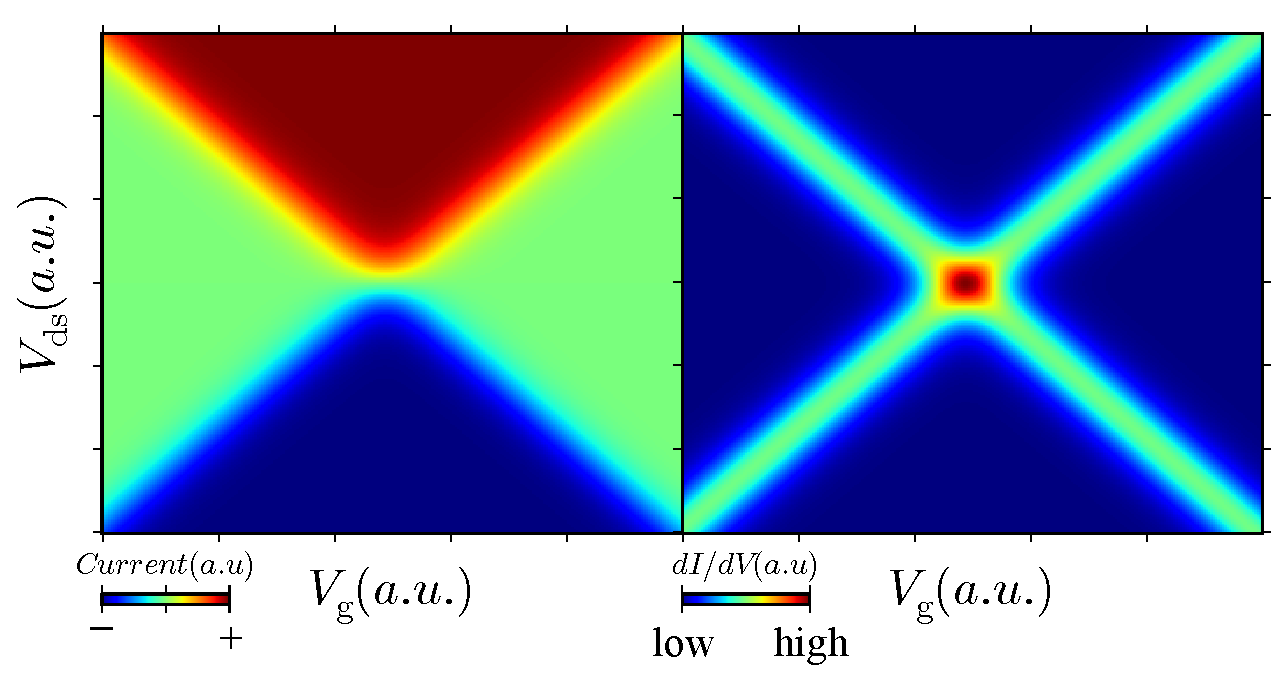
\includegraphics[scale=0.5]{Annexes/figure1/figure4.pdf} 
\caption{Courant correspant à un état de charge (0,1) dans le plan ($V_g$,$V_{ds}$) sans champ magnétique}
\label{SimulatedCoulombMap}
\end{center}
\end{figure}

\subsubsection{Quelques remarques}
Il convient toutefois de faire quelques remarque sur cette méthode des équation pilote. Tout d'abord, nous n'avons pas tenu compte des relaxation à l'intérieur de l'il\^ot. Pour inclure de tel phénomène, il faudrait introduire des taux de transfert du type $\Gamma_{\pm \rightarrow \mp}$. De plus, afin que dans le cas d'un système isoler le système retrouve une distibution de type Bolzman, il faudra s'assurer que ces deux taux de transvers obéisse à la relation suivante :
\begin{eqnarray}
\frac{\Gamma_{+ \rightarrow -}}{\Gamma_{- \rightarrow +}} = \exp(\frac{\mu_{+}- \mu_{-}}{k_bT}) \nonumber
\end{eqnarray}

Deuxième remarque, l'élargissement des niveau au sein de l'il\^ot n'est pas pris en compte. Dans le régime fortement bloqué que nous avons choisi comme modèle ici, cette hypothèse est raisonnable. 

Troisième remarque, la méthode de l'équation pilote n'est valable que dans le cas d'évènement de tunnel des électron indépendant les uns de autres. Cette méthode ne peut donc pas \^etre utiliser dans le traitement du cotunneling que l'on verra plus loin.
